\documentclass[submit,12pt]{aiaa-pretty} %submit, draft, journal options can be used
\usepackage[belowskip=0pt, aboveskip=0pt]{subcaption}
\usepackage{float}
\usepackage{caption}
\usepackage{tcolorbox}
%\setlength{\belowcaptionskip}{-10pt}

%\usepackage{classdiagram}
%\usepackage[T1]{fontenc}

\usepackage{amsmath}
\newenvironment{rcases}
  {\left.\begin{aligned}}
  {\end{aligned}\right\rbrace}
\newenvironment{lcases}
  {\left\lbrace\begin{aligned}}
  {\end{aligned}\right.}

\usepackage{amssymb}
\usepackage{amsfonts}
% * <komahan.cool@gmail.com> 2018-04-24T04:09:52.446Z:
%
% > }
%
% ^.
\usepackage{multirow}
\usepackage{booktabs}
\usepackage{doi}
\usepackage{xcolor}
\usepackage{graphicx,dblfloatfix} 
\usepackage{algorithm}
\usepackage{algpseudocode}
%\usepackage[superscript]{cite}
\usepackage[numbers,compress,sort]{natbib}
%
\usepackage{soul,xcolor}

\usepackage{amsmath}
\usepackage{amssymb}
\usepackage[normalem]{ulem}  %for italicized text

\setcounter{secnumdepth}{4} % section, subsec, subsubsection, para, subpara
\usepackage{chngcntr}
%\counterwithout{paragraph}{subsubsection} % removes paragraph from the subsubsections
\counterwithin{paragraph}{subsection} % makes paragraph depend on chapter
%\renewcommand{\theparagraph}{\arabic{paragraph}} % redefine the display of the paragraph
% Numbering of subsubsection
% https://tex.stackexchange.com/questions/3177/how-to-change-the-numbering-of-part-chapter-section-to-alphabetical-r
%\renewcommand\thesubsubsection{(\Alph{subsubsection})}
\renewcommand{\theparagraph}{(\alph{paragraph})}
%\renewcommand{\theparagraph}{\arabic{paragraph}}
%%     \arabic (1, 2, 3, ...)
%%     \alph (a, b, c, ...)
%%     \Alph (A, B, C, ...)
%%     \roman (i, ii, iii, ...)
%%     \Roman (I, II, III, ...)
%%     \fnsymbol (∗, †, ‡, §, ¶, ...)

%\usepackage[standard-baselineskips]{cmbright}
%\renewcommand\familydefault{\sfdefault}
%\usepackage[T1]{fontenc}
%\usepackage{textcomp}
% https://latex.org/forum/viewtopic.php?t=29038
%\usepackage{mathtools}
%\usepackage{amssymb}
%\usepackage{amsfonts}
%\usepackage{amsmath}

%\usepackage{eucal}
%\usepackage[mathcal]{eucal}
\usepackage[mathscr]{eucal}
\usepackage[sans]{dsfont}

%\usepackage{newtxmath}
%\SetSymbolFont{largesymbols}{bold}{OMX}{cmsy}{b}{n}

\usepackage{mathalfa}
\DeclareMathAlphabet\mathbfcal{OMS}{cmsy}{b}{n}

\usepackage{multirow}
\usepackage{booktabs}
\usepackage{doi}
\usepackage{xcolor}
\usepackage{graphicx,dblfloatfix} 
\usepackage{algorithm}
\usepackage{algpseudocode}
\usepackage{cancel}

\usepackage{bm} % load after fonts
\usepackage{epigraph} % quotes in chapter
\renewcommand{\textflush}{flushepinormal}

\usepackage{subcaption}

% Define inner product in latex
\newcommand\inner[2]{{\Bigg\langle} #1 ~\Bigg|~ #2 {\Bigg\rangle}}
\newcommand\sinner[2]{{\Big\langle} #1 ~\Big|~ #2 {\Big\rangle}}
\newcommand\linner[2]{{\big\langle} #1 ~\big|~ #2 {\big\rangle}}
\newcommand\oinner[2]{{\langle} #1 ~|~ #2 {\rangle}}
\newcommand\otinner[3]{{\langle} #1 |#2| #3 {\rangle}}
\newcommand\cinner[2]{{\langle} #1 | #2 {\rangle}}
\newcommand\crinner[2]{{(} #1 | #2 {)}}

% Define commands
\newcommand{\half}{\ensuremath{\frac{1}{2}}}

\newcommand{\bea}{\begin{eqnarray}}
\newcommand{\eea}{\end{eqnarray}}
\newcommand{\beq}{\begin{equation}}
\newcommand{\eeq}{\end{equation}}
\newcommand{\bed}{\begin{displaymath}}
\newcommand{\eed}{\end{displaymath}}

\newcommand{\pd}[2]{\dfrac{\partial #1}{\partial #2}}
\newcommand{\pf}[2]{\dfrac{d #1}{d #2}}
\newcommand{\pdt}[2]{\dfrac{\partial^2 #1}{\partial #2^2}}
\newcommand{\pft}[2]{\dfrac{d^2 #1}{d #2^2}}
\newcommand{\pdtno}[2]{\dfrac{\partial^2 #1}{\partial #2}}
\newcommand{\pdd}[3]{\dfrac{\partial^2 #1}{\partial #2 \partial #3}}
\newcommand{\pff}[3]{\dfrac{d^2 #1}{d #2 d #3}}
\newcommand{\tdt}[2]{\dfrac{d^2 #1}{d #2^2}}
\newcommand{\td}[2]{\dfrac{d #1}{d #2}}
\newcommand{\mb}{\bm}

\newcommand{\x}{\bm{x}}
\newcommand{\y}{\bm{y}}
\newcommand{\z}{\bm{z}}

\newcommand{\q}{\bm{q}}
\renewcommand{\u}{\bm{u}}
\renewcommand{\v}{\bm{v}}
\newcommand{\qd}{\bm{\dot{q}}}
\newcommand{\qdd}{\bm{\ddot{q}}}
\newcommand{\R}{\bm{R}}
\renewcommand{\S}{\bm{S}}
\newcommand{\zerovec}{\bm{0}}

\newcommand{\for}{\mathrm{for}}

\graphicspath{{figures/}}

%% \newcommand\spmatrix[1]{{%
%%   \tiny\arraycolsep=0.3\arraycolsep\ensuremath{\begin{pmatrix}#1\end{pmatrix}}}}
%% \newcommand\sbmatrix[1]{{%
%%   \tiny\arraycolsep=0.3\arraycolsep\ensuremath{\begin{bmatrix}#1\end{bmatrix}}}}
%% 

\newcommand\bdot[1]{\overset{\bm \cdot}{#1}}
% {\langle} #1 | #2 | #3 {\rangle}

\usepackage{lscape}

%  vector
\newcommand*{\vv}[1]{\vec{\mkern0mu#1}}


\graphicspath{{talk/}{talk/figures/}{figures/}}

\title{Isogeometric Finite Element Analysis Using Non-uniform Rational Bsplines}
\author{Komahan Boopathy  and Siddarth Niranjan Babu\\
  {\normalsize\itshape School of Aerospace Engineering, Georgia Institute of Technology,
    Atlanta, GA, USA. } %, 30332-0150, USA.}\\
} 

\begin{document}
\maketitle

%\abstract{}

\section{Introduction and Motivation}
Non-uniform Rational B-Splines (NURBS) \cite{Piegl:NurbsBook} are a
popular way to represent curves and surfaces in geometry modeling. In
other words, they provide a basis for three-dimensional euclidean
space. In principle, they can be used to span other spaces as well,
for example, N-dimensional vector spaces in finite element
analysis. This realization has led to the development of isogeometric
analysis
(IGA)~\cite{HUGHES20054135,KACPRZYK201487,NGUYEN201589,Agrawal2018,Milic2013}
where the same functions used for geometry representation in $\mathbb{E}^3$ is also used
to represent displacement field in $\mathbb{R}^M$.
\subsection{Importance of IGA}
\begin{itemize}
  \item FEM utilizes the approximate form of CAD geometry by discretizing them into a smaller sub-geometry called elements. Whereas in IGA, CAD-based NURBS described geometries are directly employed in the analysis without making any geometrical approximations like in FEM.
  \item IGA reduces the burden of mesh regeneration and thus minimizes the computational cost. % to a great extent.
  \item Due to inherent higher order continuity and exact representation of geometrical features, IGA has been shown to be advantageous in contact, fluid, structural vibration problems and more. 
  \item IGA can be applied to specific problems which have been solved with FEM to attain improved solution.
\end{itemize}

-- integration of geometry and analysis into a common framework


-- Isogeometric boundary element methods for elastostatic analysis were presented in [127,118],
demonstrating that mesh generation can be completely circumvented by using CAD discretizations for analysis.

R.N. Simpson, S.P.A. Bordas, J. Trevelyan, T. Rabczuk, A two-dimensional isogeometric boundary element method for elastostatic analysis,
Comput. Methods Appl. Mech. Engrg. 209–212 (2012) 87–100.

M.A. Scott, R.N. Simpson, J.A. Evans, S. Lipton, S.P.A. Bordas, T.J.R. Hughes, T.W. Sederberg, Isogeometric boundary element analysis
using unstructured T-splines, Comput. Methods Appl. Mech. Engrg. 254 (2013) 197–221.

\section{Framework}
The main objective of the project is implementation of NURBS based Isogeometric Analysis(IGA) within the existing Finite element code architecture. IGA is a recently introduced technique that employs the Computer Aided Design concepts of Non-uniform Rational B-splines(NURBS) tool to bridge the substantial  bottleneck between the CAD and finite element analysis field. The fundamental concept of IGA is to utilize the NURBS basis functions not only for the construction or as a handler of the exact form of CAD geometries, but also as a tool that can be used for their mathematical analysis. To describe the application of IGA, a standard infinite plate with a circular hole problem in tension as shown in Figure~\ref{fig:iga-demo} is chosen. 
\begin{figure}[h] 
  \centering
  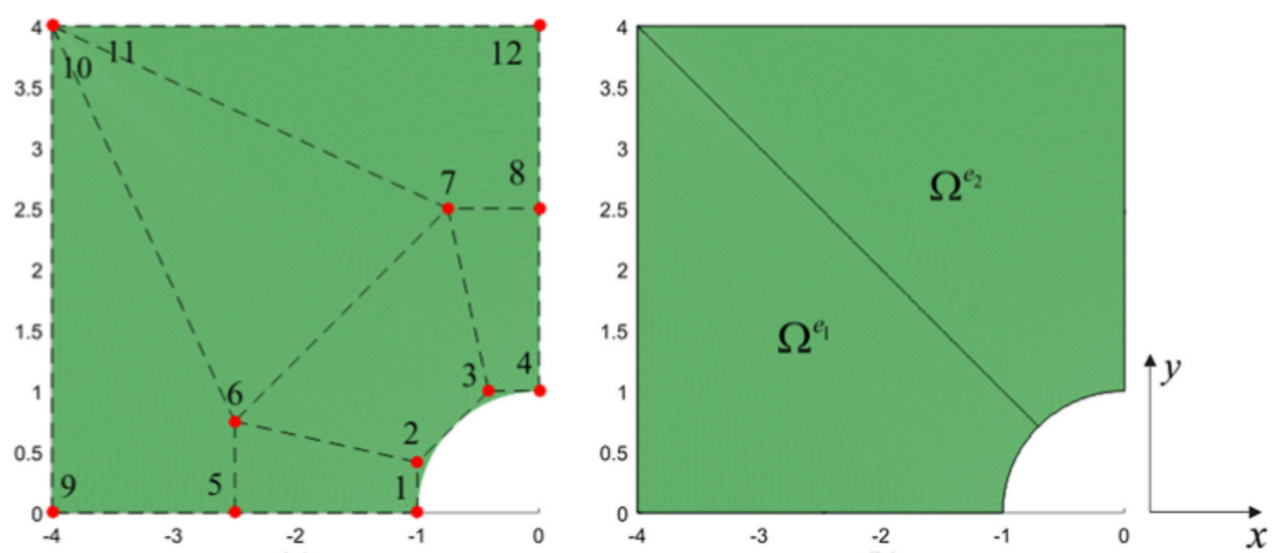
\includegraphics[width=0.5\linewidth]{iga-demo.pdf}
  \caption{\emph{NURBS decretized quarter-plate with a hole}}
  \label{fig:iga-demo}
\end{figure}
In IGA, apart from the geometrical details(length, height, width) of a
model, its parametric details such as knot vectors , the order of
NURBS basis functions, and the control points are also needed to
construct the exact form of discretized geometry. The evaluation of
NURBS basis functions and their respective derivatives, along with
their corresponding mappings are need to be done along with the
enforcement procedure for different boundary conditions for NURBS
defined geometry. The combinations of these complete the processing
stage for the proposed implementation of IGA within the FEA structure.

\subsection{Parametric Representation of Curves}
Let $\vv{p}(u) = [x(u), y(u), z(u)]^T$ refer to the parametric
representation of a point on a curve in three-dimensional Euclidean
space $\mathbb{E}^3$, where $u \in [u_{min}, u_{max}]$ is a scalar
parameter that takes a given range of values to characterize the curve. 
Any point on the curve can be written as:
\begin{equation}
  \vv{p}(u) := {\sum_{i=0}^n \alpha_i N_{k,i}(u) \vv{P}^{i}}/{\sum_{i=0}^n \alpha_i N_{k,i}(u)} \quad 0 \le u \le n-k+2
\end{equation}
where $k$ refers to the order of the $i-$th BSpline basis functions $N_{k,i}$, 
$\vv{P}^i$ is the $i-$th control point,  $n+1$ is the number of control points
and $\alpha_i$ is the weight associated with $i-th$ control point. 
The inputs required  are 
\begin{enumerate}
\item a given set of $n+1$ control points $\{\vv{P}^i\}_{i=0}^n$ and 
\item chosen order $k$
\item weights $\alpha_i$
\end{enumerate}
Note that the order is chosen independent of the number of control
points. The first-derivative (slope) of the curve at a parametric point $u$ is defined as:
\begin{equation}
  \begin{aligned}
    \td{\vv{p}(u)}{u} := \vv{p}^u(u) & = \sum_{i=0}^n  \alpha_i \td{N_{k,i}(u)}{u} \vv{P}^{i} / \sum_{i=0}^n \alpha_i \td{N_{k,i}(u)}{u}  \\ &= \sum_{i=0}^n \alpha_i N_{k,i}^{u}(u) \vv{P}^{i} /\sum_{i=0}^n \alpha_i N_{k,i}^{u}(u).
  \end{aligned}
\end{equation}
where $N_{k,i}^u(u)$ is the u-derivative of the corresponding basis
function. Here, we simply use the fact that only the basis function is
dependent on the parameter $u$. This naturally extends to second-order
derivatives (curvature) as
\begin{equation}
  \begin{aligned}
    \tdt{\vv{p}(u)}{u} := \vv{p}^{uu}(u) & = \sum_{i=0}^n \alpha_i \tdt{N_{k,i}(u)}{u} \vv{P}^{i}/\sum_{i=0}^n \alpha_i \tdt{N_{k,i}(u)}{u} \\ & = \sum_{i=0}^n \alpha_i N_{k,i}^{uu}(u) \vv{P}^{i}/\sum_{i=0}^n \alpha_i N_{k,i}^{uu}(u).
  \end{aligned}
\end{equation}
We note the following important properties of the Bspline curve:
\begin{enumerate}
\item The range of the parameter values is $0 \le u \le n-k+2$
\item The curve $\vv{p}(u)$ is $C^{k-2}$ continuous
\item $\vv{p}(u)$ is a composite curve made up of (n-k+2) segements
\item Each segment is influenced by $k$ control points
\item A given control point affects upto $k$ segments
\item If the starting and ending control points are the same $\vv{P}^0  = \vv{P}^{n+1}$, then the curve $\vv{p}(u)$ is indeed a closed curve
\end{enumerate}
The form of the NURBS basis function is
\begin{equation}
  N_{k,i}(u) = \frac{(u-t_i) N_{k-1,i}(u)}{t_{k+i-1}-t_i} + \frac{(t_{k+i}-u)N_{k-1,i+1}(u)}{t_{k+i}-t_{i+1}}
\end{equation}
where $t_i$ are the knot values defined as 
\begin{equation}
  t_i =
  \begin{cases}
    0 & i < k\\
    i+1 - k & k \le i \le n \\
    n+2 - k & i > n\\ 
  \end{cases}
\quad \forall i = 0,\ldots, n+k.
\end{equation}
It can be seen that there are a total of $n+k+1$ knot values. We can
implement a function $\texttt{knot\_values(n,k)}$ that computes the
knot values with $n$ and $k$ as inputs. The computed knot values can
be used to compute the basis function $N_{k,i}$ in a recusive manner.
The recursion is terminated when
\begin{equation}
  N_{0,i}(u) = 
  \begin{cases}
    1 & t_i \le u \le t_{i+1}    \\
    0 & \mathrm{otherwise} \\
  \end{cases}
\end{equation}

\subsection{Parametric Representation of Surfaces}

We extend the parametric curves to represent surfaces as
\begin{equation}
  \vv{p}(u_1, u_2) := \dfrac{ {\sum\limits_{i=0}^{n} \sum\limits_{j=0}^{m} \alpha_i N_{k,i}(u_1) \beta_j M_{l,j}(u_2) \vv{P}^{i,j}}} {\sum\limits_{i=0}^{n} \sum\limits_{j=0}^{m} \alpha_i N_{k,i}(u_1) \beta_j M_{l,j}(u_2)}
\end{equation}
with parameter range $0 \le u_1 \le n - k + 2$ and $0 \le u_2 \le n - l + 2$. 
For ease of notation we define the following form
\begin{equation}
  \vv{p}(\vv{u}) := \dfrac{ {\sum \limits_{s=0}^{n \times m} \alpha_{s} N_{k,s}(\vv{u}) \vv{P}^{s}}} {\sum \limits_{s=0}^{n \times m} \alpha_{s} N_{k,s}(\vv{u})}
\end{equation}

\section{Isogeometric Analysis of Bar}
\section{Isogeometric Analysis of Plate}


\section{Results}

\section{Conclusions}
\bibliographystyle{myabbrvnat} \bibliography{references}

\end{document}

